\scanpage{6}
t\rlap{e}h\rlap{h}e resolution; this \deleted{t}should not be hard whenever we have existence of resolutions in the strong sense of Hironaka, for instance in char.$0$ of if $\dim A=2$, \tikz[baseline=(s.base)]{\node[inner sep=1pt](s){I};\node[anchor=south west,inner sep=1pt](a) at ([xshift=-6em,yshift=7pt]s.north west){\inserted{\handwritten{so that two resolutions can be dominated by \unsure{-|a} third one.}}};\draw ([xshift=-4pt,yshift=-3pt]s.south west) to[out=90,in=190] ([xshift=1pt,yshift=-2pt]a.south west)--([xshift=1pt,yshift=-2pt]a.south east) to[out=0,in=-90] ([xshift=3pt,yshift=4pt]a.south east);} should point out that, in any case, the algebraic structure thus defined on $\operatorname{Pic}(U)$ depends in an essential way on the choice of the lifting of the residue field; an instructive example on which to study the dependance of this structure on the lifting is the one where $A$ is the completion of the local ring at the origin of the projecting cone of an elliptic curve (here $Q$ is isomorphic to the el liptic curve in question, for the \uline{given} lifting of $k$ ...).

I have to correct an inaccuracy that has slipped in, when defining $Q$ in the \unsure{wase|case} when $k$ is not separably closed, so as to get (10). One will then have to replace th\rlap{h}e constant group scheme $D_k$ by the twisted constant group scheme $\underline{D}$, deduced by descent from the constant group-scheme occuring after passage from $k$ to the separable closure. \figure{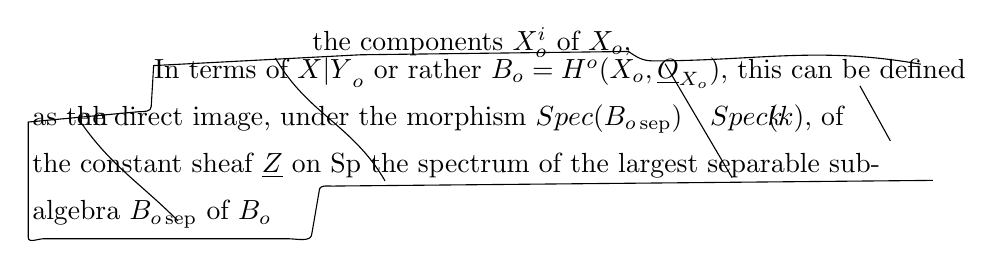
\begin{tikzpicture}[x=.44em,y=1.7em,every node/.style={anchor=base west,inner sep=0pt}]
\node at (10,0) {\deleted{In terms of \deleted{$\unsure{X|Y}_o$ or rather $B_o=H^o(X_o,\underline{O}_{X_o})$}, this can be defined}};
\node at (23,.60) {\deleted{\inserted{the components $X_o^i$ of $X_o$,}}};
\node at (0,-1) {\deleted{as t\rlap{e}h\rlap{h}e direct image, under the morphism $\operatorname{Spec}(B_{o\,\mathrm{sep}})\quad \operatorname{Spec}\mathord{\rlap{$k$}(}k)$, of}};
\node at (0,-2) {\deleted{the constant sheaf $\underline{Z}$ on \deleted{Sp} the spectrum of the largest separable sub-}};
\node at (0,-3) {\deleted{algebra $B_{o\,\mathrm{sep}}$ of $B_o$}};
\draw (73,.31) to[out=170,in=0] (51,.38) to[out=180,in=-35] (49,.58)--(27,.51)--(10,.28)--(9.8,-.59) to[out=-90,in=0] (8.8,-.70)--(-.3,-.92)--(-.3,-3.37) to[out=-90,in=180] (1,-3.40)--(21,-3.40) to[out=0,in=-90] (23,-3.28)--(23.6,-2.38) to[out=90,in=185] (25,-2.28)--(74,-2.16);
\draw (4,-.92) to[out=-55,in=135] (12,-3.02);
\draw (20,.44) to[out=-60,in=120] (29,-2.17);
\draw (52,.32)--(57.5,-2.10);
\draw (68,-.15)--(70.5,-1.32);
\end{tikzpicture}} This can be made explicit, in terms of the separable algebraic closures \deleted{of} $k_i$ of $k$ in the function fiel\tikz[baseline=(s.base)]{\node[inner sep=0pt](s){d};\fill ([xshift=-1pt,yshift=2pt]s.north west) circle (.3pt);}e of the irreducible components $X_o^i$ of $X_o$, as the \deleted{product of the schemes} direct image of the constant sheaf $\underline{Z}$ under the projection $\operatorname{Spec}(\handwritten{\prod}k_i)\handwritten{\longrightarrow}\operatorname{Spec}(k\unsure{)}$

To study the inverse system $(P_n)$, use the fact (SGA 6 XII) that the \deleted{\unsure{s}}transition morphisms are affine, which gives a sense to $P=\underset{\handwritten{\longleftarrow}}{\lim}P_n$ as an actual group-scheme. It's Lie algebra is the inverse limit of the Lie algebras \rlap{H}of the $P_n$, which are $H^1(X_n,\underline{O}_{X_n})$, therefore we get
% archive sheet number: 5
